\documentclass[10pt,mathserif]{beamer}
\usetheme{Madrid}

\title[Asma y AQ]{Impacto de la Contaminación Atmosférica en los Casos de Asma en California}
\author{Grupo Morado}
\date{Enero 2026}

\usepackage{xspace}


% --- DATA SOURCES ---
\newcommand{\openaq}{\texttt{OpenAQ}\xspace}
\newcommand{\datagov}{\texttt{data.gov}\xspace}
\newcommand{\bboxt}{\texttt{bbox}\xspace}

\begin{document}
    \begin{frame}
        \titlepage
    \end{frame}
    \begin{frame}
        \frametitle{Contenido}
        \tableofcontents[hideallsubsections]
    \end{frame}

    \section{Descripción del Proyecto}\label{sec:descripcion-del-proyecto}
    \begin{frame}
        \frametitle{Motivación}
        \begin{figure}
            \centering
            \includegraphics[width=200pt]{../tex/figures/one_earth_poster}
            \caption{Portada del artículo de One Earth~\cite{Ni2024PM25Asthma}}
            \label{fig:one_earth_poster}
        \end{figure}
    \end{frame}
    \begin{frame}
        \frametitle{Motivación}
        \pause
        \begin{itemize}
            \item Negligencia de repercusiones ambientales
            \vfill\pause
            \item Impacto sobre enfermedades respiratorias
            \vfill\pause
            \item Aumento de la prevalencia del asma
            \vfill\pause
            \item Intensificación de ataques de asma
            \vfill\pause
            \item Caso de estudio: California
        \end{itemize}
    \end{frame}

    \begin{frame}
        \frametitle{Objetivos}
        \pause
        \begin{itemize}
            \item Recopilar datos históricos
            \vfill\pause
            \item Evaluar estado actual (\textit{WHO guidelines}~\cite{who2021_global_aqg})
            \vfill\pause
            \item Evaluar cobertura de estaciones de monitoreo
            \vfill\pause
            \item Análisis en relación con la incidencia de asma
            \vfill\pause
            \item Proponer medidas
            \vfill\pause
            \item Modelo predictivo de ingresos hospitalarios
        \end{itemize}
    \end{frame}

    \begin{frame}
        \frametitle{Requisitos}
        \pause
        \begin{itemize}
            \item Datos
            \vfill\pause
            \item Herramientas y Software
            \vfill\pause
            \item Recursos humanos
            \vfill\pause
            \item Recursos materiales
            \vfill\pause
            \item Organización temporal
        \end{itemize}
    \end{frame}

    \section{Gestión del proyecto}\label{sec:gestion-del-proyecto}
    \begin{frame}
        \frametitle{Paquetes de trabajo}
        \begin{figure}
            \centering
            \includegraphics[width=1\linewidth]{../management/WBS}
            \caption{Esquema de Paquetes de Trabajo (WBS)}
            \label{fig:wbs}
        \end{figure}
    \end{frame}
    \begin{frame}
        \frametitle{Fase 2: Recopilación de Datos}
        \begin{center}
            \includegraphics[height=0.85\textheight]{../management/WBS-fase-2}
        \end{center}
    \end{frame}
    \begin{frame}
        \frametitle{Cronograma}
        \begin{center}
            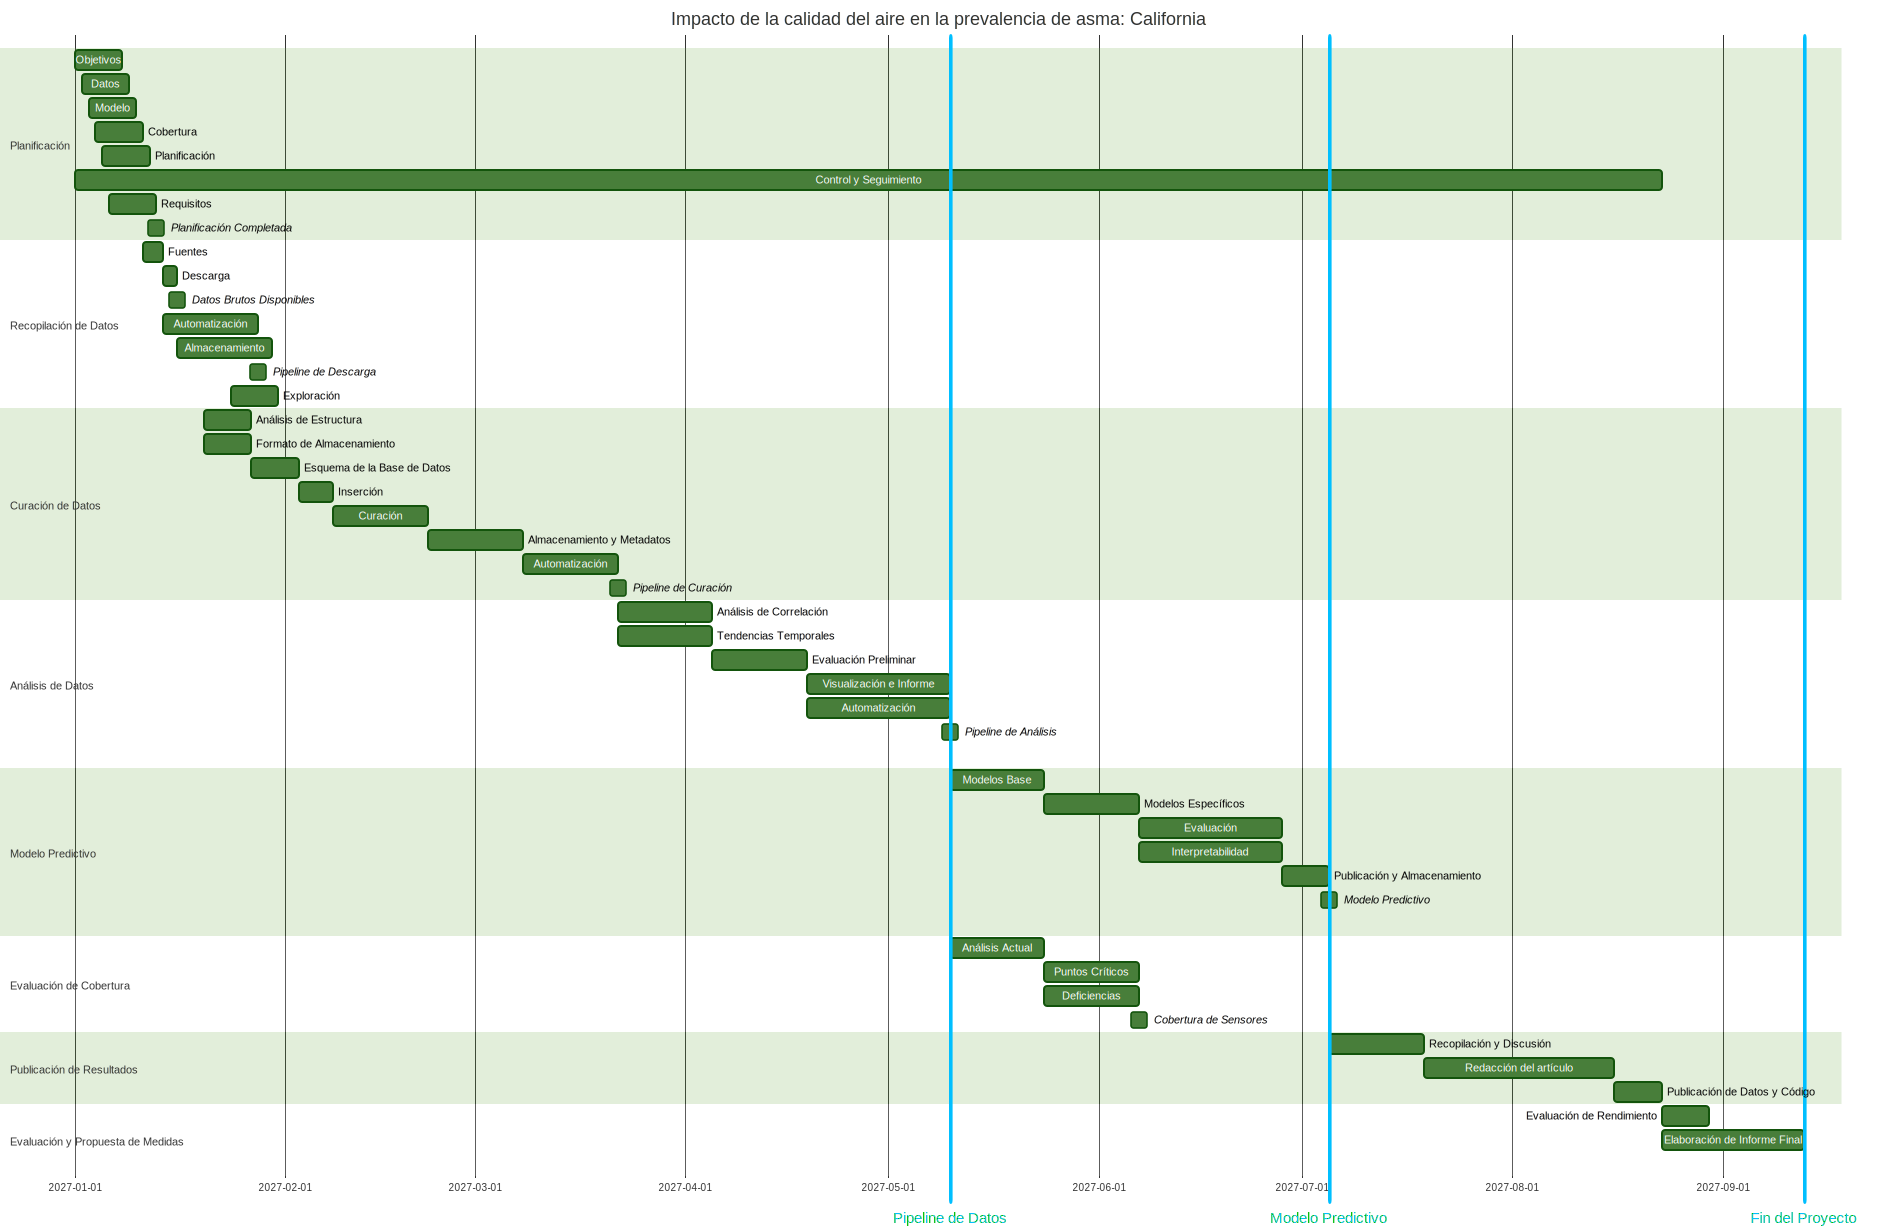
\includegraphics[height=0.85\textheight]{../management/Gantt}
        \end{center}
    \end{frame}
    \begin{frame}
        \frametitle{Cronograma}
        \begin{center}
            \includegraphics[height=0.85\textheight]{../management/gantt-focus-5-6}
        \end{center}
    \end{frame}

    \section{Plan de Preservación de Datos}\label{sec:plan-de-preservacion-de-datos}

    % --- PARTE DE SAMUEL
    % Diapositiva 1: Filosofía General
    \begin{frame}
        \frametitle{Estrategia de Preservación: Principios FAIR}
        \begin{block}{Objetivo}
            Garantizar la integridad, disponibilidad y reutilización de los activos digitales a largo plazo (10-20 años).
        \end{block}

        \vspace{0.5cm}

        \begin{columns}
            \begin{column}{0.5\textwidth}
                \textbf{Principios FAIR:}
                \begin{itemize}
                    \item \textbf{F}indable (Encontrable)
                    \item \textbf{A}ccessible (Accesible)
                    \item \textbf{I}nteroperable
                    \item \textbf{R}eusable (Reutilizable)
                \end{itemize}
            \end{column}
            \begin{column}{0.5\textwidth}
                \textbf{Acciones Clave:}
                \begin{itemize}
                    \item Documentación con \textit{Dublin Core}.
                    \item Licencia abierta \textbf{CC-BY 4.0}.
                    \item Uso de identificadores persistentes (\textbf{DOI}).
                \end{itemize}
            \end{column}
        \end{columns}
    \end{frame}

    % Diapositiva 2: Seguridad (La parte visualmente más importante)
    \begin{frame}
        \frametitle{Seguridad e Integridad de los Datos}

        \begin{alertblock}{Política de Backup: Regla 3-2-1}
            Mitigación de fallos de hardware y \textit{ransomware}.
        \end{alertblock}

        \vspace{0.3cm}

        \begin{enumerate}
            \item \textbf{3 Copias} de los datos en todo momento.
            \item \textbf{2 Soportes} distintos (SSD local + HDD externo).
            \item \textbf{1 Copia Remota} (\textit{Off-site} en Nube Institucional).
        \end{enumerate}

        \vspace{0.5cm}
        \pause

        \textbf{Mecanismos de Defensa:}
        \begin{itemize}
            \item \textbf{Air Gap:} Discos HDD desconectados físicamente cuando no se usan (Defensa anti-virus).
            \item \textbf{Hashing:} Verificación de huella digital para detectar \textit{bit rot} (deterioro silencioso de datos).
        \end{itemize}
    \end{frame}

    % Diapositiva 3: Transformación para el Futuro
    \begin{frame}
        \frametitle{Preservación a Largo Plazo}
        \textit{Migración proactiva para evitar la obsolescencia tecnológica.}

        \vspace{0.5cm}

        \begin{table}
            \centering
            \begin{tabular}{l | l}
                \textbf{Fase Activa (Propietario)} & \textbf{Archivo Definitivo (Abierto)} \\
                \hline
                \hline
                Microsoft Excel (.xlsx) & \textbf{CSV (UTF-8)} \\
                ArcGIS Pro (.aprx, .shp) & \textbf{GeoJSON} \\
                Word / Docs & \textbf{PDF/A} (ISO 19005) \\
                Google Drive & \textbf{Zenodo (CERN)} \\
            \end{tabular}
            \caption{Estrategia de migración de formatos}\label{tab:table}
        \end{table}

        \pause
        \begin{itemize}
            \item \textbf{Repositorio Final:} Zenodo.
            \item \textbf{Garantía:} Inmutabilidad asegurada por el CERN durante +20 años.
        \end{itemize}
    \end{frame}


    % -- PARTE DE JULIO

    % --- VISTA GENERAL DEL PLAN ---
    \begin{frame}{DMP: Horizon Europe Template}
        \begin{columns}
            \column{0.5\textwidth}
            \centering
            \vspace{0.2cm}
            \includegraphics[width=\textwidth]{figures/image_20b5c9}

            \column{0.5\textwidth}
            \centering
            \vspace{0.2cm}
            \includegraphics[width=\textwidth]{figures/image_20b604}
        \end{columns}
    \end{frame}

    \begin{frame}
    	\frametitle{Metadatos: Estándar Dublin Core}
    	\begin{center}
            \includegraphics[height=0.85\textheight]{../management/dc-metadata}
    	\end{center}
    \end{frame}

    \section{Fuentes de datos}\label{sec:fuentes-de-datos}
    \subsection{\openaq}\label{subsec:openaq}
    \begin{frame}
        \frametitle{\openaq}
        \begin{center}
            \includegraphics[width=50pt]{figures/openaq_icon}
        \end{center}
            \pause
        \begin{center}
            \includegraphics[width=200pt]{figures/openaq_leaflet_usa}
        \end{center}
    \end{frame}

    \begin{frame}
        \frametitle{Contaminantes}
        \pause
        \begin{itemize}
            \item $\pmtwofive$~\cite{Khreis2017TRAPchildhoodAsthma}
            \vfill\pause
            \item $\pmten$~\cite{Khreis2017TRAPchildhoodAsthma}
            \vfill\pause
            \item $\notwo$~\cite{Khreis2017TRAPchildhoodAsthma,Naidoo2019NO2asthma}
            \vfill\pause
            \item $\ozone$~\cite{epa2025_ozone_asthma_health_effects}
        \end{itemize}
    \end{frame}

    \begin{frame}
        \frametitle{Geometría de los condados}
        Shapefiles de los condados de California~\cite{census_tiger2025_us_county}
        \pause
        \begin{center}
            \includegraphics[width=200pt]{../tex/figures/us_counties_qgis}
        \end{center}
    \end{frame}

    \begin{frame}
        \frametitle{Geometría de los condados}
        \begin{center}
            \includegraphics[width=150pt]{../tex/figures/california_counties_qgis}
        \end{center}
    \end{frame}

    \begin{frame}
        \frametitle{API de \openaq}
        \begin{itemize}
            \item \textit{Bounding Box} de California
            \vfill
            \pause
            \item Límite de peticiones por minuto: 60
            \vfill
            \item Límite de peticiones por hora: 2000
            \vfill
            \pause
            \item Número de peticiones a realizar: 5333
        \end{itemize}
        
        \bigskip\pause
        
        \begin{center}
            \textbf{¡2 a 3 horas de ejecución!}
        \end{center}
    \end{frame}

    \subsection{\datagov}\label{subsec:data-gov}
    \begin{frame}
        \frametitle{\datagov}
        \begin{itemize}
            \item Prevalencia de asma (CHIS, \textit{California Health Interview Survey}~\cite{cdph_asthma_prevalence_datagov})
            \vfill\pause
            \item Agregaciones
            \begin{itemize}
                \vfill
                \item Grupo demográfico
                \vfill
                \item Condado
                \vfill
                \item Bianual
            \end{itemize}
        \end{itemize}
    \end{frame}
    
    \subsection{Base de datos integrada}\label{subsec:base-de-datos-integrada}
    \begin{frame}
        \frametitle{Base de datos integrada}
        \begin{center}
            \includegraphics[width=200pt]{../data/openaq_data/sensors/unified phase 2}
        \end{center}
    \end{frame}

    \section{Análisis de datos}\label{sec:analisis-de-datos}
    \begin{frame}
        \frametitle{Niños con asma vs. $\notwo$}
        \begin{center}
            \includegraphics[width=0.85\linewidth]{../code/figures/ranked_counties_2016__NO__2___Child_vs__adult__0_17_years}
        \end{center}
    \end{frame}

    \begin{frame}
        \frametitle{Niños con asma vs. $\ozone$}
        \begin{center}
            \includegraphics[width=0.85\linewidth]{../code/figures/ranked_counties_2016__O__3___Child_vs__adult__0_17_years}
        \end{center}
    \end{frame}

    \begin{frame}
        \frametitle{Niños con asma vs. $\pmtwofive$}
        \begin{center}
            \includegraphics[width=0.85\linewidth]{../code/figures/ranked_counties_2016__PM___2_5____Child_vs__adult__0_17_years}
        \end{center}
    \end{frame}
    
    \begin{frame}
    	\frametitle{Niños con asma vs. $\pmten$}
        \begin{center}
            \includegraphics[width=0.85\linewidth]{../code/figures/ranked_counties_2016__PM___10____Child_vs__adult__0_17_years}
        \end{center}
    \end{frame}

    \begin{frame}
        \frametitle{Población total con asma vs. $\pmtwofive$}
        \begin{center}
            \includegraphics[width=0.85\linewidth]{../code/figures/ranked_counties_2016__PM___2_5____Total_population__All_ages}
        \end{center}
    \end{frame}

    \bibliographystyle{plainurl}
    \bibliography{bibliography}
\end{document}